\section{What is calculus? Why are you learning it?}

The word \emph{calculus} comes from Latin, literally meaning `small pebble' which frankly isn't too far off from the actual concerns of calculus. Simply put, calculus asks two main questions:

\begin{quest}[The Two Main Questions of Calculus]\label{mainquestion}\leavevmode
	\begin{enumerate}
		\item What does a small change in one thing tell you about change in something else?
		\vspace{2mm}
		\item How do these small changes add up to give a sum?
	\end{enumerate}
\end{quest}

We will approach the first of these questions using \emph{differentiation} and the second with another concept called \emph{integration}. As we will see, these two questions are intimately related, and we'll be able to find a very useful relationship between differentiation and integration.

Before we begin trying to unpack and answer these two questions, I'm sure you must be forming two of your own?
\begin{quest}
Why am I learning this?	Why is any of this useful?
\end{quest}

Differentiation and integration have numerous applications in statistics, physics, chemistry, biology, economics, and generally are useful for understanding how things change in the world around us. In fact, some of the things in the world around you (like your brain, car, and phone) are already using calculus and its principles which we will explore through caes studies.

Calculus is used to calculate energy and motion in physics, reaction rates and radioactive decay in chemistry, birth and death rates in biology, and costs and revenues in economics. In many cases, calculus is the natural language for describing a problem. Let's start with one such example where the central ideas of calculus naturally appear.

\begin{exmp}
Suppose two people $M$ and $J$ are having a race from a point $a$ to another point $b$. When watching this sort of thing play out, we develop a vague idea or prediction of the winner is going to be. In order to come to a conclusion, we unconsciously ask ourselves questions like ``Where are $M$ and $J$?'' and ``How fast are they running?''. To answer the first, we simply recall where they were at a particular time $t^*$. This method doesn't work as well when it comes to the second, how can we remember their speed right at time $t^*$? Let's take a step back and look at where they were at different points in the race.

\begin{figure}[h]\label{fig:Race}
\centering
\begin{subfigure}{\textwidth}
  \centering
  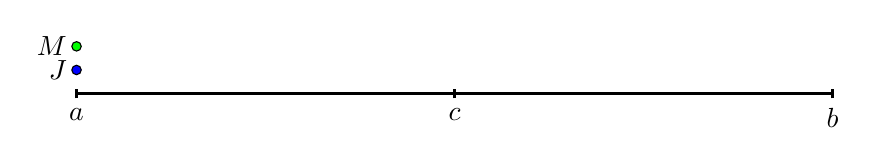
\begin{tikzpicture}[scale=.6]
      \draw [very thick] (0,0)-- (16,0);
  		\draw [thick] (0,-.1) node[below]{$a$} -- (0,0.1);
  		\draw [thick] (16,-.1) node[below]{$b$} -- (16,0.1);
  		\draw [thick] (8,-.1) node[below]{$c$} -- (8,0.1);
  		\draw [fill=blue] (0,.5) circle [radius=0.1]
  		node[left] (0, .5) {$J$};
  		\draw [fill=green] (0,1) circle [radius=0.1]
  			node[left] (0, 1) {$M$};
  	\end{tikzpicture}\hspace{12pt}
\end{subfigure}

\begin{subfigure}{\textwidth}
  \centering
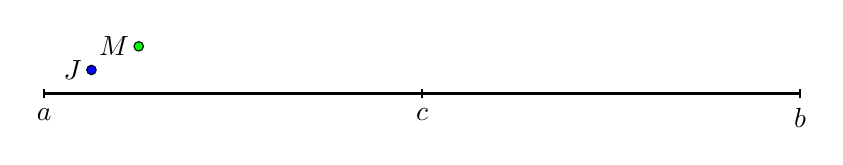
\begin{tikzpicture}[scale=.6]
	\draw [very thick] (0,0)-- (16,0);
	\draw [thick] (0,-.1) node[below]{$a$} -- (0,0.1);
	\draw [thick] (16,-.1) node[below]{$b$} -- (16,0.1);
	\draw [thick] (8,-.1) node[below]{$c$} -- (8,0.1);
	\draw [fill=blue] (1,.5) circle [radius=0.1]
	node[left] (1, .5) {$J$};
	\draw [fill=green] (2,1) circle [radius=0.1]
		node[left] (2, 1) {$M$};
\end{tikzpicture}
\end{subfigure}

\begin{subfigure}{\textwidth}
  \centering
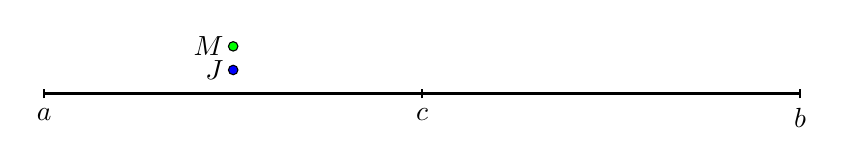
\begin{tikzpicture}[scale=.6]
	\draw [very thick] (0,0)-- (16,0);
	\draw [thick] (0,-.1) node[below]{$a$} -- (0,0.1);
	\draw [thick] (16,-.1) node[below]{$b$} -- (16,0.1);
	\draw [thick] (8,-.1) node[below]{$c$} -- (8,0.1);
	\draw [fill=blue] (4,.5) circle [radius=0.1]
	node[left] (4, .5) {$J$};
	\draw [fill=green] (4,1) circle [radius=0.1]
		node[left] (4, 1) {$M$};
\end{tikzpicture}
\end{subfigure}


\begin{subfigure}{\textwidth}
  \centering
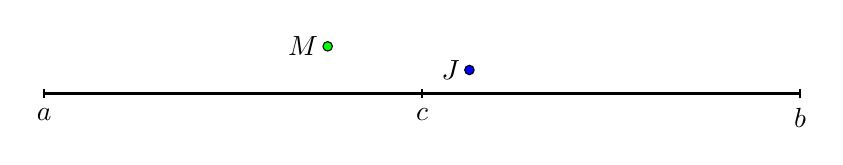
\begin{tikzpicture}[scale=.6]
	\draw [very thick] (0,0)-- (16,0);
	\draw [thick] (0,-.1) node[below]{$a$} -- (0,0.1);
	\draw [thick] (16,-.1) node[below]{$b$} -- (16,0.1);
	\draw [thick] (8,-.1) node[below]{$c$} -- (8,0.1);
	\draw [fill=blue] (9,.5) circle [radius=0.1]
	node[left] (9, .5) {$J$};
	\draw [fill=green] (6,1) circle [radius=0.1]
	node[left] (6, 1) {$M$};
\end{tikzpicture}
\end{subfigure}

\begin{subfigure}{\textwidth}
  \centering
  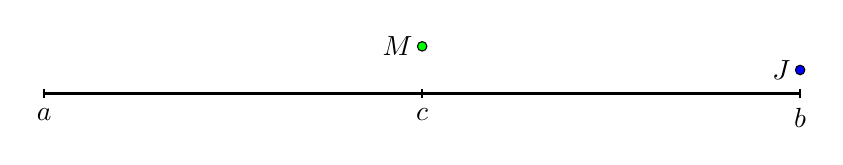
\begin{tikzpicture}[scale=.6]
	\draw [very thick] (0,0)-- (16,0);
	\draw [thick] (0,-.1) node[below]{$a$} -- (0,0.1);
	\draw [thick] (16,-.1) node[below]{$b$} -- (16,0.1);
	\draw [thick] (8,-.1) node[below]{$c$} -- (8,0.1);
	\draw [fill=blue] (16,.5) circle [radius=0.1]
	node[left] (16, .5) {$J$};
	\draw [fill=green] (8,1) circle [radius=0.1]
	node[left] (8, 1) {$M$};
\end{tikzpicture}
\end{subfigure}
\caption{Visualizing the race}
\end{figure}

If we look at \cref{fig:Race}, we see an example of a race like this. In this case, $J$ wins the race in 5 seconds and $M$ loses it, so intuitively, $J$ must have moved faster than $M$. We can attempt to capture this using the average speed formula

\begin{equation}
	\text{Average Speed}=\frac{\text{Distance Traveled}}{\text{Time}}.
\end{equation}
   If we call the speed of $M$ $v_M$ and the speed of $v_J$, then $M$ and $J$ have speeds
\begin{equation}
v_M=\frac{c-a}{5}\ \text{and}\ v_J=\frac{b-a}{5}.
\end{equation}

This confirms our intuition that $J$ was faster at the end of the day, but something is missing here. At the start of the race, $J$ is behind $M$ and moving slower, so $J$ must have began to speed up. Therefore, it's incorrect to say that $J$ is moving at speed $v_J$ at every point in time. Let's try a different approach. First, we visualize the race by graphing both runners' position at every point in race.

\begin{figure}
  \hspace{-5mm}
\begin{subfigure}{0.35\textwidth}
  \centering
  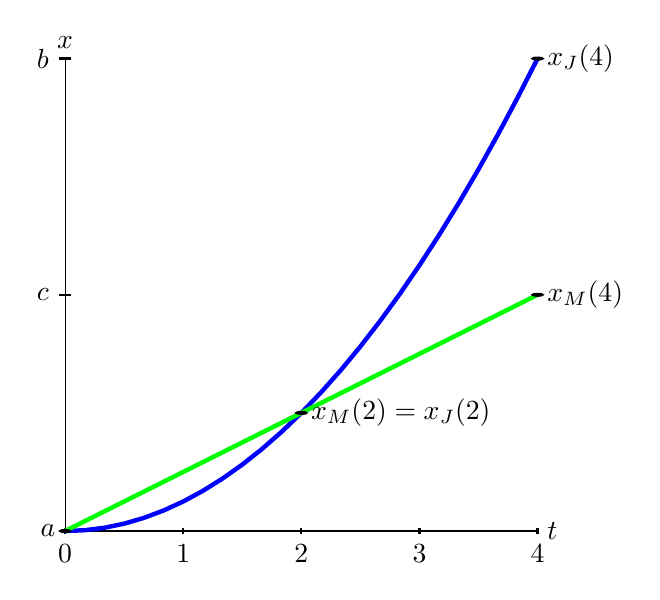
\begin{tikzpicture}[yscale=0.375, xscale=1.5]
\draw (0,16) -- (0,0) -- (4,0);
	\node [left] at (0,0) [left] {$a$};
		\draw [thick] (-0.05,8) node[left]{$c$} -- (0.05,8);
		\draw [thick] (-0.05,16) node[left]{$b$} -- (0.05,16);

		\draw [thick] (0,-0.1) node[below]{$0$} -- (0,0.1);
		\draw [thick] (1,-0.1) node[below]{$1$} -- (1,0.1);
		\draw [thick] (2,-0.1) node[below]{$2$} -- (2,0.1);
		\draw [thick] (3,-0.1) node[below]{$3$} -- (3,0.1);
		\draw [thick] (4,-0.1) node[below]{$4$} -- (4,0.1);

	\node [right] at (4,0) [right] {$t$};
  \node [above] at (0,16) [above] {$x$};


	\draw[blue, ultra thick, domain=0:4] plot (\x, {\x*\x});

	\draw[green, ultra thick, domain=0:4] plot (\x, {2*\x});

	\node at (2,4) [right] {$x_M(2)=x_J(2)$};
	\node at (4,8) [right] {$x_M(4)$};
	\node at (4,16) [right] {$x_J(4)$};

	\draw[fill] (0,0) circle [radius=0.05];
	\draw[fill] (2,4) circle [radius=0.05];
	\draw[fill] (4,8) circle [radius=0.05];
	\draw[fill] (4,16) circle [radius=0.050];
\end{tikzpicture}
\end{subfigure}
\hspace{35mm}
\begin{subfigure}{0.35\textwidth}
  \centering
  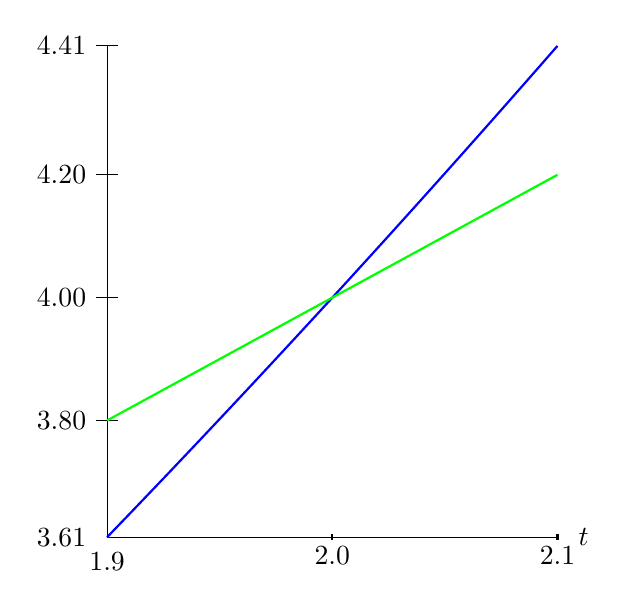
\begin{tikzpicture}[scale=13, yscale=0.6, xscale=2.2]
  	\draw (1.9, 4.41)-- (1.9,3.61)-- (2.1,3.61);

  	\node at (1.9, 3.6) [below] {$1.9$};
  	\node at (2, 3.61) [below] {$2.0$};
  	\node at (2.1, 3.61) [below] {$2.1$};
  	\node at (1.895, 3.61) [left] {$3.61$};
  	\node at (1.895, 3.8) [left] {$3.80$};
  	\node at (1.895, 4) [left] {$4.00$};
  	\node at (1.895, 4.2) [left] {$4.20$};
  	\node at (1.895, 4.41) [left] {$4.41$};
  	\node at (2.105, 3.61) [right] {$t$};


  \draw (1.895, 3.8)-- (1.905, 3.8);
  \draw (1.895, 4)-- (1.905, 4);
  \draw (1.895, 4.2)-- (1.905, 4.2);
  \draw (1.895, 4.41)-- (1.905, 4.41);
  \draw[thick] (2, 3.605)-- (2, 3.615);
  \draw[thick] (2.1, 3.605)-- (2.1, 3.615);


  	\draw[blue, thick, domain=1.9:2.1] plot (\x, {\x*\x});
  	\draw[green, thick, domain=1.9:2.1] plot (\x, {2*\x});
  \end{tikzpicture}
\end{subfigure}



\caption{Graph of time $t$ v. position $x$ at different scales.}
\end{figure}


From this, we see that the positions of $M$ and $J$ are functions of time. If we're given a point in the race $t$, we can find their positions $x_M(t)$ and $x_J(t)$ using functions $x_M$ and $x_J$. This allows us to rephrase the question. If we want to figure out how fast $M$ and $J$ moving at $t^*$, we need to see how their position functions change around that time. In short, we want the \text{rate of change} of $x_M$ and $x_J$ around $t^*$. In algebra 1 or 2, you learn to calculate rate of change as the slope $m$ of a line $y=mt+b$.
\begin{equation*}
	m = \frac{\text{Change in}\ y  }{\text{Change in}\ t} = \frac{\Delta y}{\Delta x}.
\end{equation*}
We'll write these changes as $\Delta y$ and $\Delta t$. If we zoom in on our functions $x_J$ and $x_M$ far enough, we see that they look straight lines. This allows us to look at small differences in $t$, $x_M$, and $x_J$. Let's say $x_M(2.1)=4.2$, $x_M(1.9)=3.8$, $x_M(2.1)=4.41$, and $x_M(1.9)= 3.61$. If we try to approximate the rate of change this way, then the velocity of $M$ and $J$ at $t^*=2$ are approximately given by: \begin{align}
	v^*_M\approx&\frac{\Delta x_M}{\Delta t}=\frac{4.2-3.8}{2.1-1.9}=\frac{0.4}{0.2}=2\\
	v^*_J\approx&\frac{\Delta x_J}{\Delta t}=\frac{4.41-3.61}{2.1-1.9}=\frac{0.8}{0.2}=4.
\end{align}

We now know that if we zoom in very close and look at small differences, then we're able to approximate how something is changing at a particular moment. This is the same idea behind how a car's speedometer calculates the speed of the car. Calculus comes in when we try to make this method more generally applicable.
\end{exmp}
